\section{Results}
\subsection{Forecast accuracy}
The models score the same 8,760 hours in 2023 and 8,784 in 2024.
Lasso had the lowest 2023 MAE and RMSE, while boosting led on the
eligible hit rate. Boosting had the lowest 2024 MAE and RMSE and the
highest eligible hit rate among the five reported configurations
(Table~\ref{tab:forecast}).

\begin{table}[!t]
\centering
\caption{Annual MAE and RMSE (EUR/MWh), and \(\pm5\%\) hits (\%).
Eligible hours: 7,738 in 2023 and 7,620 in 2024.}
\label{tab:forecast}
\setlength{\tabcolsep}{3pt}
\begin{tabular}{lrrrrrr}
\hline
& \multicolumn{3}{c}{2023} & \multicolumn{3}{c}{2024}\\
Model & MAE & RMSE & Hit & MAE & RMSE & Hit\\
\hline
Ridge & 18.78 & 26.65 & 20.35 & 18.34 & 29.52 & 17.80\\
Lasso & 17.91 & 26.14 & 21.85 & 17.84 & 29.35 & 18.75\\
Forest & 21.00 & 30.50 & 20.65 & 18.98 & 31.56 & 18.31\\
Boosting & 18.39 & 26.87 & 22.87 & 16.58 & 27.47 & 19.09\\
MLP & 20.22 & 27.79 & 16.81 & 19.19 & 30.07 & 16.08\\
\hline
\end{tabular}
\end{table}

\textbf{Lasso.} Tuning reduced MAE from 20.65 to 17.91 in 2023
and from 19.14 to 17.84 in 2024. The pre-2023 fit retained about
77 of 604 inputs per hour model. At negative prices in 2024, Lasso
scored 19.79 MAE and Ridge 19.43.
The chosen Lasso took about 140 seconds to fit over 24 refits,
compared with about 3 seconds for Ridge on the same laptop. Raising
the starter's iteration limit changed its fixed-window validation
RMSE only from 31.028 to 31.030 EUR/MWh.

\textbf{Random Forest.} Using the validation-selected leaf size of two
gave MAE 20.86 and 18.91, each within 1\% of the reported leaf-five
setting. The forest's large-error rate was highest in the high-price
regime in both years (16.67\% and 13.43\%), across only 11 and 18 days.
The evening-peak group produced by splitting that regime at \(k=5\)
also had the highest large-error rate in both years.

\textbf{Gradient Boosting.} The absolute-loss variant reached a
20.70\% hit rate in 2024, after losing on 2023 MAE and hit count.
Boosting's 2024 MAE on negative prices was 20.69, above Ridge's 19.43.

\textbf{MLP.} Tuning lowered MAE from 22.46 to 20.22 in 2023
and from 20.37 to 19.19 in 2024. The remaining gap to Ridge
averaged about 2.0 EUR/MWh in the overnight and late-evening bands
and 0.6 during 07:00--19:59.
The tuned MLP beat Ridge in two months of 2023 and six of 2024,
even though its annual MAE was higher in both years. Increasing
the starter's iteration budget changed its MAE by only 0.005 EUR/MWh.

\subsection{Regimes and rule transfer}
The four-cluster fit had a training Davies--Bouldin index of 1.29.
In 2024, large Ridge errors exceeded 40.54 EUR/MWh and occurred
in 8.96\% of hours. Autumn evenings had 92 events in 546 hours.
Cluster-0 afternoons had 72 in 786 hours. Within the afternoon
band, the Ridge event rate was 9.16\% for cluster 0 and 11.28\%
for other clusters, a difference of \(-2.12\) percentage points
(95\% block interval \([-8.33,3.50]\)).

\begin{figure}[!t]
\centering
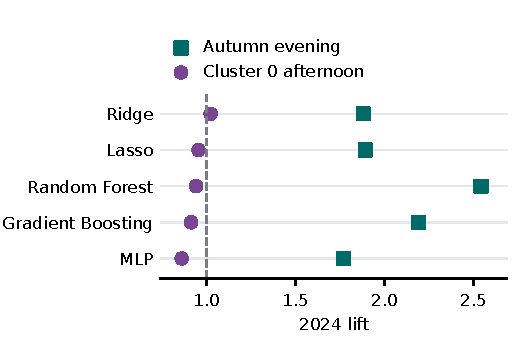
\includegraphics[width=\columnwidth]{Figures/rule_transfer.pdf}
\caption{2024 lift for two antecedents selected on 2023 Ridge errors.
Each model uses its own frozen 2023 large-error threshold. Lift 1
denotes the model's annual large-error rate.}
\label{fig:rule-transfer}
\end{figure}

Across all five models, autumn-evening lift was 1.77--2.54 and
cluster-0 afternoon lift was 0.86--1.02 (Fig.~\ref{fig:rule-transfer}).
The same qualitative pattern held using the common Ridge threshold.
Under model-specific thresholds, the annual large-error rate for
boosting was 6.27\%, and its autumn-evening rate was 13.74\%
(75 of 546 hours). Ridge's autumn-evening rate was 16.85\%, against
its higher annual rate of 8.96\%. Lift therefore compares enrichment
relative to each model's reference rate.
For boosting, autumn-evening lift (2.19) exceeded autumn alone
(1.55) and evening alone (1.40). Its highest-lift rules mined
separately on 2023 boosting errors fell to 0.75 and 0.97 in 2024.
